\documentclass{standalone}
% This file was created with tikzplotlib v0.9.15.

\usepackage{siunitx}
\usepackage{pgfplots}
% and optionally (as of Pgfplots 1.3):
\pgfplotsset{compat=newest}
\pgfplotsset{plot coordinates/math parser=false}
\newlength\figureheight
\newlength\figurewidth

\newcommand{\Set}[1]{\mathcal{#1}}
\newcommand{\Vector}[1]{\bm{\MakeLowercase{#1}}}
\newcommand{\Operator}[1]{\bm{\MakeUppercase{#1}}}
%%%%%%%%%%
\DeclareMathAlphabet{\mathsfbr}{OT1}{cmss}{m}{n}%for math sans serif (cmss)
\SetMathAlphabet{\mathsfbr}{bold}{OT1}{cmss}{bx}{n}%for math sans serif (cmss)
\DeclareRobustCommand{\msf}[1]{%
  \ifcat\noexpand#1\relax\msfgreek{#1}\else\mathsfbr{#1}\fi%for math sans serif (cmss)
}
\DeclareFontEncoding{LGR}{}{} % or load \usepackage{textgreek}
\DeclareSymbolFont{sfgreek}{LGR}{cmss}{m}{n}
\SetSymbolFont{sfgreek}{bold}{LGR}{cmss}{bx}{n}
\DeclareMathSymbol{\sXi}{\mathalpha}{sfgreek}{`X}
\DeclareMathSymbol{\sUpsilon}{\mathalpha}{sfgreek}{`U}

\begin{document}
% This file was created with tikzplotlib v0.9.15.
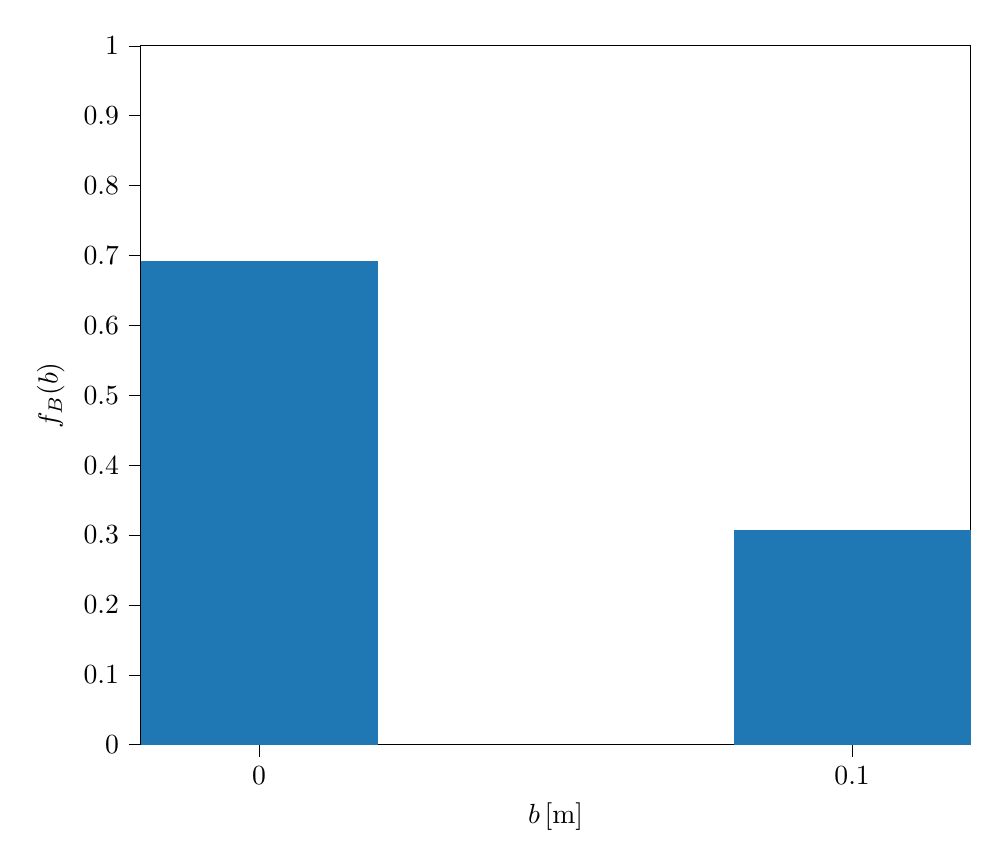
\begin{tikzpicture}

\definecolor{color0}{rgb}{0.12156862745098,0.466666666666667,0.705882352941177}
% \definecolor{color0}{blu}

\begin{axis}[
width=1\linewidth,
tick align=outside,
tick pos=left,
x grid style={white!69.0196078431373!black},
xlabel={$b \left[ \si{m} \right]$},
xmin=-0.02, xmax=0.12,
xtick={0.00,0.10},
xtick style={color=black},
y grid style={white!69.0196078431373!black},
ylabel={$f_{\msf{B}}(b)$},
ymin=0, ymax=1,
ytick style={color=black},
% ytick={0,1000,2000,3000,4000,5000,6000,7000,8000},
ytick={0.0,0.1,0.2,0.3,0.4,0.5,0.6,0.7,0.8,0.9,1}
]
\draw[draw=none,fill=color0] (axis cs:-0.02,0) rectangle (axis cs:0.02,0.6921);
\draw[draw=none,fill=color0] (axis cs:0.08,0) rectangle (axis cs:0.12,0.3079);
\end{axis}

\end{tikzpicture}
\end{document}